\documentclass[12pt,a4paper,landscape]{article}
\usepackage[icelandic]{babel}
\usepackage[T1]{fontenc}
\usepackage[utf8]{inputenc}
\usepackage{multicol}
\usepackage{calc}
\usepackage{amsmath}
\usepackage{pgf,tikz}
\usepackage{mathrsfs}
\usetikzlibrary{arrows,decorations.text}
\usepackage{array}
\usepackage{eso-pic}
\usepackage{graphicx}
\usepackage{pxfonts}
\usepackage{enumitem}
\usepackage{comment}


% If you're reading this, be prepared for confusion.  Making this was
% a learning experience for me, and it shows.  Much of the placement
% was hacked in; if you make it better, let me know...

\DeclareFixedFont{\sf}{T1}{phv}{b}{n}{0.11mm}



\newcommand*\punktur{%
\makebox[\fontcharwd\font`.][c]{%
\resizebox{\fontcharht\font`.}{!}{
\begin{tikzpicture}[%
                                             decoration={%
                                               reverse path,%
                                               text along path,%
                                               text={|\sffamily\color{gray}\huge| Benedikt Bjarni Bogason --},%
                                               }%
                                           ]%
                                           \draw [decorate] (0,0) circle (1.7);%
                                           \fill[color=black] (0,0) circle (1.5);%
                                           \end{tikzpicture}%
                                    }%
                                }%
                    }%

% All this page size stuff is a hack, but it seems to work
% Turn off header and footer
\pagestyle{empty}

\setlength{\oddsidemargin}{0.05in}
\setlength{\evensidemargin}{0.5in}
\setlength{\textwidth}{10in}


\setlength{\topmargin}{-0.65in}
\setlength{\textheight}{7.25in}
\setlength{\headheight}{0in}
\setlength{\headsep}{0in}



 

% Redefine section commands to use less space
\makeatletter
\renewcommand{\section}{\@startsection{section}{1}{0mm}%
                                {-1ex plus -.5ex minus -.2ex}%
                                {0.5ex plus .2ex}%x
                                {\normalfont\Large\bfseries}}
\renewcommand{\subsection}{\@startsection{subsection}{2}{0mm}%
                                {-1explus -.5ex minus -.2ex}%
                                {0.5ex plus .2ex}%
                                {\normalfont\small\bfseries}}
\renewcommand\subsubsection{\@startsection{subsubsection}{3}{0mm}%
                                {-1ex plus -.5ex minus -.2ex}%
                                {1ex plus .2ex}%
                                {\normalfont\small\bfseries}}
\makeatother

% Define BibTeX command
\def\BibTeX{{\rm B\kern-.05em{\sc i\kern-.025em b}\kern-.08em
    T\kern-.1667em\lower.7ex\hbox{E}\kern-.125emX}}

% Don't print section numbers
\setcounter{secnumdepth}{0}


\setlength{\parindent}{0pt}
%\setlength{\parskip}{0pt plus 0.5ex}
\setlength{\parskip}{0.5pt}

% -----------------------------------------------------------------------
\makeatletter
  \AddToShipoutPicture{%
    \setlength{\@tempdimb}{.95\paperwidth}%
    \setlength{\@tempdimc}{.07\paperheight}%
    \setlength{\unitlength}{1pt}%
    \put(\strip@pt\@tempdimb,\strip@pt\@tempdimc){%
      \mbox{\rotatebox{90}{\scriptsize \copyright~Fjölbrautaskólinn í Garðabæ\punktur~~Gjört 2017\!\punktur}}
    }
}
\makeatother

% -----------------------------------------------------------------------

\begin{document}
\begin{center}
     \Large{\textbf{Formúlublað}} \\
\end{center}

\raggedright
\footnotesize
\begin{multicols}{3}


% multicol parameters
% These lengths are set only within the two main columns
%\setlength{\columnseprule}{0.25pt}
\setlength{\premulticols}{1pt}
\setlength{\postmulticols}{1pt}
\setlength{\multicolsep}{1pt}
\setlength{\columnsep}{2pt}

%\subsection{Vaxtareikningar}
%	\begin{multicols}{2}
%		\begin{align*}
%    			v   &= H  p  t    \\
%   			H_n &= H (1 \pm p)^n 
%		\end{align*}
%		\begin{align*}
%			H_n &= H \left( 1 + \frac{p}{m}\right)^{mn}	\\
%			H_n &= H e^{pn}
%		\end{align*}
%	\end{multicols}
%
\subsection{Rétthyrndur þríhyrningur} 
\vspace{2mm}
	\begin{multicols}{3}
		\begin{align*}
			\cos v &= \dfrac{\text{\scriptsize Aðl}}{\text{\scriptsize Lang}}
		\end{align*}
		\begin{align*}
			\sin v &= \dfrac{\text{\scriptsize Mótl}}{\text{\scriptsize Lang}}
		\end{align*}
		\begin{align*}
			\tan v &= \dfrac{\text{\scriptsize Mótl}}{\text{\scriptsize Aðl}}
		\end{align*}
	\end{multicols}
\vspace{2mm}
%
\subsection{Jafna beinnar línu}
	\begin{multicols}{2}
		\begin{align*}
			y &= hx + k 
		\end{align*}
     		\begin{align*}
			y - y_1 &= h(x - x_1)
		\end{align*}
	\end{multicols}
%
\subsection{Fjarlægðarformúla}
	\begin{align*}
		d &= \sqrt{(x_2 - x_1)^2 + (y_2 - y_1)^2}
	\end{align*}
% 
\subsection{Hallatala línu}
	\begin{align*} 
		h = \frac{\Delta y}{\Delta x} = \frac{y_2 - y_1}{x_2 - x_1} 
	\end{align*}
%
\subsection{Miðpunktur striks}
	\begin{align*} 
		M   = \left( \dfrac{x_1 + x_2}{2}, \dfrac{y_1 + y_2}{2} \right)
	\end{align*}
%
\subsection{Lausnaformúla}
	\begin{align*} 
		x = \dfrac{-b \pm \sqrt{b^2 - 4ac}}{2a}
	\end{align*}
%
\subsection{Samhverfuás}
	\begin{align*} 
		x = \dfrac{-b}{2a}
	\end{align*}
%
\begin{comment}
\subsection{Kósínusregla}
    \[ c^2 = a^2 +b^2 -2ab\cos C \]
\subsection{Sínusregla}
\[ \dfrac{\sin A}{a} = \dfrac{\sin B}{b} = \dfrac{\sin C}{c}  \]
\subsection{Flatarmálsregla}
\[ F = \dfrac{a b \sin C}{2} \]
\end{comment}
%
\subsection{Lograr}
	\begin{multicols}{2}
		\begin{align*}
			\lg(A B) &= \lg A + \lg B
		\end{align*}
		\begin{align*}
			\lg \left( \frac{A}{B} \right) &= \lg A - \lg B
		\end{align*}
	\end{multicols}
	\begin{align*}
		\lg A^y &= y\lg A
	\end{align*}
%
\subsection{Umraðanir og samantektir}
	\begin{align*}
		P(n,k) &= \frac{n!}{(n-k)!} \\
		C(n,k) &= \dbinom{n}{k} = \frac{P(n,k)}{k!} = \frac{n!}{(n-k)!k!}
	\end{align*}
%
\subsection{Hornaföll}
	\begin{align*}
		\sin(u \pm v) &= \sin u \cdot \cos v \pm \cos u \cdot \sin v \\
		\cos(u \pm v) &= \cos u \cdot \cos v \mp \sin u \cdot \sin v \\[0.5em]
		\sin 2u &= 2\sin u \cdot \cos u \\
		\cos 2u &= \cos^2 u - \sin^2 u \\[0.5em]
		1 &= \cos^2 u + \sin^2 u \\
		\tan u &= \frac{\sin u}{\cos u}
	\end{align*}
%
\subsection{Vigrar}
	\begin{align*}
		\vec{u} \cdot \vec{v} &= |\vec{u}|\cdot |\vec{v}| \cdot \cos(\vec{u},\vec{v})
%		|\vec{u} \times \vec{v}| &= |\vec{u}|\cdot |\vec{v}| \cdot \sin(\vec{u},\vec{v}) 
	\end{align*}
%
\subsection{Afleiður}
	\begin{align*}
		f'(x) &= \lim_{h \to 0}\dfrac{f(x+h) - f(x)}{h} = \lim_{x \to x_0}\dfrac{f(x) - f(x_0)}{x - x_0} \\[0.5em] 
		(f\cdot g)' 	&= f' \cdot g + f \cdot g'		\\[0.5em]
		\left(\dfrac{f}{g}\right)' &= \dfrac{f'\cdot g - f\cdot g'}{g^2} 
	\end{align*}
%
\subsection{Keðjuregla}
	\begin{align*}
		\big( f(g(x)) \big)' = f'(g(x)) \cdot g'(x)
	\end{align*}
%
\subsection{Töluleg heildun}
	\begin{align*}
		T &= \frac{f(x_1) + f(x_2)}{2} \cdot h  \\[0.5em]
		M &= f(m) \cdot h                   \\[0.5em]
		S   &= \frac{T+2M}{3}
	\end{align*} 
%
\subsection{Runur og raðir}
	\begin{multicols}{2}
		\begin{align*}
			a_n &= a_1 + (n-1) d             \\
			a_n &= a_1 \cdot k^{n-1}              \\
			s   &= \frac{a_1}{1-k} \\
		\end{align*}
		\begin{align*}
			s_n &= \frac{n(a_1 + a_n)}{2}    \\
			s_n &= \frac{a_1(k^n - 1)}{k-1}
	\end{align*}
\end{multicols}
%
\subsection{Hlutheildun}
	\begin{align*}
		%\int f(x) g'(x)~dx = f(x)g(x) - \int f'(x)g(x)~dx
		\int f(x) g(x)~dx = f(x)G(x) - \int f'(x)G(x)~dx
	\end{align*} 
%
\subsection{Rúmmál}
	\begin{align*}
		V_x     &= \pi \int_a^b \big( f(x) \big)^2\,dx                                          \\
		V_x     &= \pi \int_a^b \bigg( \big(f(x) \big)^2 - \big(g(x) \big)^2 \bigg)\,dx         \\
		V_{y=k} &= \pi \int_a^b \big( f(x) - k\big)^2\,dx                                       \\
		V_y     &= 2\pi \int_a^b x\big|f(x)\big|\,dx                                            \\
		V_y     &= 2\pi \int_a^b x\big|f(x) - g(x)\big|\,dx                                     \\
		V_{x=k} &= 2\pi \int_a^b (x-k)\big|f(x) - g(x)\big|\,dx \qquad \text{ef $k \leq a < b$}
	\end{align*}
%
\subsection{Bogalengd}
	\begin{align*}
		s &= \int_a^b \sqrt{1 + (f'(x))^2}\,dx  
	\end{align*}
%
\subsection{Yfirborðsflatarmál}
	\begin{align*}
		Y_x &= 2\pi\int_a^b \big| f(x) \big| \sqrt{1 + (f'(x))^2}\,dx                           \\
		Y_y &= 2\pi\int_a^b \big| x \big| \sqrt{1 + (f'(x))^2}\,dx                           
	\end{align*}
%
\subsection{Tvinntölur}
	\begin{align*}
		P(z) &= \left( z^2 - 2{\rm Re}(w)\cdot z + |w|^2 \right) \cdot Q(z) \\
		e^{ix} &= \cos x + i \sin x 
	\end{align*}
%
\subsection{Deildajöfnur}
	\begin{align*}
		y &= k_1 e^{\alpha_1 x} + k_2 e^{\alpha_2 x}    \\
		y &= e^{px} (k_1 \cos(qx) + k_2 \sin(qx))    \\
		y &= e^{\alpha x} (k_1x + k_2)    
\end{align*}
%


%\rule{0.45\linewidth}{0.25pt}
%\scriptsize
%
%Gjört 2007\\ 
%Fjölbrautaskólinn í Garðabæ

\end{multicols}
\clearpage

\begin{center}
     \Large{\textbf{Formúlublað}} \\
\end{center}

\raggedright
\footnotesize
\begin{multicols}{3}


% multicol parameters
% These lengths are set only within the two main columns
%\setlength{\columnseprule}{0.25pt}
\setlength{\premulticols}{1pt}
\setlength{\postmulticols}{1pt}
\setlength{\multicolsep}{1pt}
\setlength{\columnsep}{2pt}



\newcommand\bbbPic{2.5cm}




\subsection{Þríhyrningur}
\begin{tabular}{ m{5cm}  m{2.4cm} }
%\hline
%%%%%%%%%%%%%%%%%%%
\begin{tikzpicture}
\coordinate (A) at (0,0);
\coordinate (B) at (1,4);
\coordinate (C) at (5,0);
\coordinate (E) at (1,0);
\draw[thick] (A) -- node[midway,left] {$c$} (B) -- node[midway,right,yshift=1mm] {$a$} (C) -- node[midway,below] {$b$} cycle;
\draw[dotted] (B) -- node[midway,right] {$h$} (E);
\draw (E) rectangle ++(0.3, 0.3);
\draw (A) node[left] {$A$};
\draw (B) node[above] {$B$};
\draw (C) node[right] {$C$};
\end{tikzpicture}
%%%%%%%%%%%%%%%%%%%
&
%\begin{minipage}[c]{2.4cm}
$F = \dfrac{a b \sin C}{2}$\\[18pt]
%$c^2 = a^2 + b^2 - 2 a b \cos C$\\[18pt]
%$\dfrac{\sin A}{a} = \dfrac{\sin B}{b}  = \dfrac{\sin C}{c} $
%\end{minipage}
\\
%\hline
\end{tabular}


\subsection{Samsíðungur}
\begin{tabular}{ m{5cm}  m{2.4cm} }
%\hline
%%%%%%%%%%%%%%%%%%%
\begin{tikzpicture}
\coordinate (A) at (0,0);
\coordinate (B) at (1,4);
\coordinate (C) at (5,4);
\coordinate (D) at (4,0);
\coordinate (E) at (1,0);
\draw[thick] (A) -- (B) -- (C) -- (D) -- node[midway,below] {$g$} cycle;
\draw[dotted] (B) -- node[midway,right] {$h$} (E);
\draw (E) rectangle ++(0.3, 0.3);
\draw (A) node[left, opacity=0] {$C$};
\draw (B) node[above, opacity=0] {$B$};
\draw (C) node[right, opacity=0] {$A$};
\end{tikzpicture}
%%%%%%%%%%%%%%%%%%%
&
$F = g  h$
\\
%\hline
\end{tabular}



\subsection{Trapisa}
\begin{tabular}{ m{5cm}  m{2.4cm} }
%\hline
%%%%%%%%%%%%%%%%%%%
\begin{tikzpicture}
\coordinate (A) at (0,0);
\coordinate (B) at (1,4);
\coordinate (C) at (4,4);
\coordinate (D) at (5,0);
\coordinate (E) at (1,0);
\draw[thick] (A) -- (B) -- node[midway,above] {$a$} (C) -- (D) -- node[midway,below] {$b$} cycle;
\draw[dotted] (B) -- node[midway,right] {$h$} (E);
\draw (E) rectangle ++(0.3, 0.3);
\draw (A) node[left, opacity=0] {$C$};
\draw (B) node[above, opacity=0] {$B$};
\draw (D) node[right, opacity=0] {$A$};
\end{tikzpicture}
%%%%%%%%%%%%%%%%%%%
&
$F=\dfrac{(a+b) h}{2}$
\\
%\hline
\end{tabular}



\subsection{Hringur}
\begin{tabular}{ m{5cm}  m{2.4cm} }
%\hline
%%%%%%%%%%%%%%%%%%%
\begin{tikzpicture}[scale=1.2]
\draw [shift={(2.,2.)}] (0.:0.3) arc (0.:42.5:0.3) node[midway,right,yshift=0.5mm] {$v$};
\draw[thick] (2.,2.) circle (2.cm);
\draw[dotted] (0.5564352570549509,0.615759835532145) -- node[midway,left,xshift=-0mm,yshift=1mm] {$\textit{þ}$} (3.464137615067828,3.362461391799229);
\draw[dotted] (2.,2.) -- node[midway,below] {$r$} (4.,2.);
\draw [shift={(2.,2.)}] (0.:2) arc (0.:42.5:2) node[midway,left] {$b$};
\fill (2,2) circle (1pt);
\end{tikzpicture}
%%%%%%%%%%%%%%%%%%%
&
\begin{minipage}[c]{2.4cm}
$U = 2 \pi r = \textit{þ} \pi$\\[18pt]
$F = \pi r^2$\\[18pt]
$b = \dfrac{v}{360^\circ} \cdot U$\\[18pt]
$F_g = \dfrac{v}{360^\circ} \cdot F$
\end{minipage}
\\
%\hline
%%%%%%%%%%%%%%%%%%%%%%%%%%%%%
\end{tabular}




\subsection{Kassi}
\begin{tabular}{ m{5cm}  m{2.4cm} }
%\hline
%%%%%%%%%%%%%%%%%%%
\begin{tikzpicture}
\coordinate (A) at (0,0);
\coordinate (B) at (0,3);
\coordinate (C) at (4,3);
\coordinate (D) at (4,0);
\coordinate (E) at (1,4);
\coordinate (F) at (5,4);
\coordinate (G) at (5,1);
\coordinate (H) at (1,1);
\draw[thick] (A) -- (B) -- (E) -- node[above,midway,opacity=0] {$filler$} (F) -- (G) node[midway,right] {$h$} -- node[midway,right,yshift=-1mm] {$b$} (D) -- node[midway,below] {$a$} cycle;
\draw[thick] (B) -- (C);
\draw[thick] (F) -- (C) -- (D);
\draw[dashed] (A) -- (H) -- (E);
\draw[dashed] (H) -- (G);
\draw (H) rectangle ++(0.3, 0.3);
\end{tikzpicture}
%%%%%%%%%%%%%%%%%%%
&
\begin{minipage}[c]{2.4cm}
$R = a b h$%\\[18pt]
%$Y = 2(ab + ah + bh)$
\end{minipage}
\\
%\hline
\end{tabular}




\subsection{Sívalningur}
\begin{tabular}{ m{5cm}  m{2.4cm} }
%\hline
%%%%%%%%%%%%%%%%%%%
\begin{tikzpicture}[scale=0.9]
\coordinate (M) at (2.5,0);
\coordinate (Q) at (2.5,3.5);
\draw[thick] [rotate around={0.:(Q)}] (Q) ellipse (2.6100766272276408cm and 0.75cm);
\draw[dashed] ((2.5,0) + (0:2.6100766272276408cm and 0.75cm) arc
  (0:180:2.6100766272276408cm and 0.75cm);
\draw[thick] ((2.5,0) + (180:2.6100766272276408cm and 0.75cm) arc
  (180:360:2.6100766272276408cm and 0.75cm);
\draw[thick] (-0.11007662722763767,3.5)-- (-0.11007662722763722,0.);
\draw[thick] (5.110076627227643,3.5)-- node[midway,right] {$h$} (5.110076627227643,0.);
\draw[dotted] (5.110076627227643,0.)-- node[midway,below] {$r$} (M);
\fill (M) circle (1pt);
\end{tikzpicture}
%%%%%%%%%%%%%%%%%%%
&
\begin{minipage}[c]{2.4cm}
$R = \pi r^2 h$ \\[18pt]
$M = 2 \pi r h$\\[18pt]
$Y = M + 2 \pi r^2$
\end{minipage}
\\
%\hline
\end{tabular}

\begin{comment}
\subsection{Strendingur}
\begin{tabular}{ m{5cm}  m{2.4cm} }
%\hline
%%%%%%%%%%%%%%%%%%%
\begin{tikzpicture}
\fill (0.,0.) circle (\bbbPic);
\end{tikzpicture}
%%%%%%%%%%%%%%%%%%%
&
$R = Gh$
\\
%\hline
\end{tabular}
\end{comment}

\subsection{Kúla}
\begin{tabular}{ m{5cm}  m{2.4cm} }
%\hline
%%%%%%%%%%%%%%%%%%%
\begin{tikzpicture}[scale=0.9]
\coordinate (M) at (2.5,0);
\draw[dashed] ((2.5,0) + (0:2.6100766272276408cm and 0.75cm) arc
  (0:180:2.6100766272276408cm and 0.75cm);
\draw[thick] ((2.5,0) + (180:2.6100766272276408cm and 0.75cm) arc
  (180:360:2.6100766272276408cm and 0.75cm);
\draw[dotted] (5.110076627227643,0.) -- node[midway,below] {$r$} (M);
\draw[thick] (M) circle (2.6100766272276434cm);
\fill (M) circle (1pt);
\end{tikzpicture}
%%%%%%%%%%%%%%%%%%%
&
\begin{minipage}[c]{2.4cm}
$R=\dfrac{4\pi r^3}{3}$\\[18pt]
$Y = 4 \pi r^2$
\end{minipage}
\\
%\hline
%%%%%%%%%%%%%%%%%%%%%%%%%%%%%
\end{tabular}


\vfill


\subsection{Pýramídi}
\begin{tabular}{ m{5cm}  m{2.4cm} }
%\hline
%%%%%%%%%%%%%%%%%%%
\begin{tikzpicture}
\coordinate (T) at (2.5,4.25);
\coordinate (A) at (0,0);
\coordinate (B) at (4,0);
\coordinate (C) at (1,1);
\coordinate (D) at (5,1);
\coordinate (Q) at (2.5,0.5);
\draw [dashed] (A)-- (C);
\draw [dashed] (C)-- (D);
\draw [dashed] (C)-- (T);
\draw [thick] (A)-- (T);
\draw [thick] (B)-- (T);
\draw [thick] (T)-- (D);
\draw [thick] (D) -- node[midway,right,yshift=-1mm] {$b$} (B);
\draw [thick] (B) -- node[midway,below] {$a$} (A);
\draw [dotted] (T) -- node[midway,right] {$h$} (Q);
\fill (Q) circle (1pt);
\end{tikzpicture}
%%%%%%%%%%%%%%%%%%%
&
$R=\dfrac{a b h}{3}$
\\
%\hline
\end{tabular}

\vfill

\subsection{Keila}
\begin{tabular}{ m{5cm}  m{2.4cm} }
%\hline
%%%%%%%%%%%%%%%%%%%
\begin{tikzpicture}[scale=0.9]
\coordinate (M) at (2.5,0);
\coordinate (T) at (2.5,4.25);
\draw[dashed] ((2.5,0) + (0:2.6100766272276408cm and 0.75cm) arc
  (5:175:2.6100766272276408cm and 0.75cm);
\draw[thick] ((2.5,0) + (180:2.6100766272276408cm and 0.75cm) arc
  (180:360:2.6100766272276408cm and 0.75cm);
\draw[thick] (-0.11007662722763722,0.) -- (T);
\draw[thick] (T) -- node[midway,right,yshift=1mm] {$s$} (5.110076627227643,0.);
\draw[dotted] (T) -- node[midway,right] {$h$} (M);
\draw[dotted] (5.110076627227643,0.)-- node[midway,below] {$r$} (M);
\fill (M) circle (1pt);
\draw (M) rectangle ++(0.3, 0.3);
\end{tikzpicture}
%%%%%%%%%%%%%%%%%%%
&
\begin{minipage}[c]{2.4cm}
$R=\dfrac{\pi r^2 h}{3}$\\[18pt]
$M = \pi r s$\\[18pt]
$Y = M + \pi r^2$
\end{minipage}
\\
%\hline
%%%%%%%%%%%%%%%%%%%%%%%%%%%%%
\end{tabular}

\end{multicols}

\clearpage

\begin{center}
     \Large{\textbf{Formúlublað}} \\
\end{center}

\raggedright
\footnotesize
\begin{multicols}{3}

% multicol parameters
% These lengths are set only within the two main columns
%\setlength{\columnseprule}{0.25pt}
\setlength{\premulticols}{1pt}
\setlength{\postmulticols}{1pt}
\setlength{\multicolsep}{1pt}
\setlength{\columnsep}{2pt}



\subsection{Deildunarreglur (Diffrun)}
\begin{itemize}[label=]
\item $\dfrac{d}{dx}~k = 0$ \quad ($k$ er fasti)
\item $\dfrac{d}{dx}~k f(x)= k \left(\dfrac{d}{dx}~ f(x)\right)$ \quad ($k$ er fasti)
\item $\dfrac{d}{dx}~(f(x) \pm g(x)) = f'(x) \pm g'(x)$
\item $\dfrac{d}{dx}~x = 1$
\item $\dfrac{d}{dx}~\sqrt{x} = \dfrac{1}{2\sqrt{x}}$
\item $\dfrac{d}{dx}~x^n = nx^{n-1}$
\item $\dfrac{d}{dx}~a^x = \ln a \cdot a^x$
\item $\dfrac{d}{dx}~|x| = \dfrac{x}{|x|}$
\item $\dfrac{d}{dx}~e^{ax} = ae^{ax}$
\item $\dfrac{d}{dx}~\sin x = \cos x$
\item $\dfrac{d}{dx}~\sin ax = a\cos ax$
\item $\dfrac{d}{dx}~\cos x = -\sin x$
\item $\dfrac{d}{dx}~\cos ax = -a\sin ax$
\item $\dfrac{d}{dx}~\tan x = \dfrac{1}{\cos^2 x} = 1 + \tan^2 x$
\item $\dfrac{d}{dx}~\tan ax = \dfrac{a}{\cos^2ax} = a(1 + \tan^2 ax)$
\item $\dfrac{d}{dx}~\ln |x| = \dfrac{1}{x}$
\item $\dfrac{d}{dx}~\ln |ax+b| = \dfrac{a}{ax+b}$
\item $\dfrac{d}{dx}~\sin^{-1} x = \dfrac{1}{\sqrt{1-x^2}}$
\item $\dfrac{d}{dx}~\cos^{-1} x = -\dfrac{1}{\sqrt{1-x^2}}$
\item $\dfrac{d}{dx}~\tan^{-1} x = \dfrac{1}{1+x^2}$
\end{itemize}

%\vfill

\subsection{Keðjuregla}
	\vspace{-4mm}
	\begin{align*}
		\dfrac{d}{dx}~ f(g(x))  = f'(g(x)) \cdot g'(x)
	\end{align*}


\subsection{Samsett föll}
	\begin{align*}
		\dfrac{d}{dx}~\big( f(x) \cdot g(x) \big) &= f'(x) \cdot g(x) + f(x) \cdot g'(x) \\
		\dfrac{d}{dx}~\left(\dfrac{f(x)}{g(x)}\right) &= \dfrac{f'(x) \cdot g(x) - f(x) \cdot g'(x)}{(g(x))^2}
	\end{align*}

\subsection{Hlutheildun}
	\begin{align*}
		\int f(u) g'(u)~du = f(u)g(u) - \int f'(u)g(u)~du
	\end{align*}


\subsection{Meðalgildi}
	\vspace{-4mm}
	\begin{align*}
		m(f) = \dfrac{1}{b-a}\int_a^b f(u)~du
	\end{align*}



\subsection{Heildunarreglur (Tegrun)}
\begin{itemize}[label=]
\item $\displaystyle\int du = u + C$
\item $\displaystyle\int k~du = ku + C$ \quad ($k$ er fasti)
\item $\displaystyle\int (du \pm dv) = \int du \pm \int dv$
\item $\displaystyle\int u^n~du = \dfrac{u^{n+1}}{n+1} + C$ \quad ($n \neq -1$)
\item $\displaystyle\int \dfrac{du}{u} = \ln\left|u\right| + C$
\item $\displaystyle\int a^u~du = \dfrac{a^u}{\ln a} + C$ \quad $a>0$, $a\neq1$
\item $\displaystyle\int e^u~du = e^u + C$
\item $\displaystyle\int e^{bu}~du = \dfrac{e^{bu}}{b} + C$ \quad ($b \neq 0$)
\item $\displaystyle\int \sin u~du = - \cos u + C$
\item $\displaystyle\int \sin bu~du = - \dfrac{\cos bu}{b} + C$ \quad ($b \neq 0$)
\item $\displaystyle\int \cos u~du = \sin u + C$
\item $\displaystyle\int \cos bu~du = \dfrac{\sin bu}{b} + C$ \quad ($b \neq 0$)
\item $\displaystyle\int \dfrac{1}{u+b}~du = \ln|u+b| + C$
\item $\displaystyle\int \dfrac{1}{au+b}~du = \dfrac{1}{a}\ln|au+b| + C$
\item $\displaystyle\int \dfrac{1}{\cos^2 u}~du = \tan u + C$
\item $\displaystyle\int \dfrac{1}{\sin^2 u}~du = -\dfrac{1}{\tan u} + C$
\item $\displaystyle\int \dfrac{\tan u}{\cos u}~du = \dfrac{1}{\cos u} + C$
%\item $\displaystyle\int \csc u \cot u~du = - \csc u + C$
\item $\displaystyle\int \tan u~du = - \ln\left|\cos u\right| + C$
\item $\displaystyle\int \dfrac{1}{\tan u}~du = \ln\left|\sin u\right| + C$
%\item $\displaystyle\int \dfrac{du}{\sqrt{a^2 - u^2}} = \sin^{-1}\left(\dfrac{u}{a}\right) + C$
\item $\displaystyle\int \dfrac{du}{a^2 + u^2} = \dfrac{1}{a} \tan^{-1}\left(\dfrac{u}{a}\right) + C$
%\item $\displaystyle\int \dfrac{du}{u\sqrt{u^2 - a^2}} = \dfrac{1}{a}\sec^{-1}\left|\dfrac{u}{a}\right| + C$
\item $\displaystyle\int \dfrac{du}{a^2 - u^2} = \dfrac{1}{2a} \ln\left|\dfrac{u+a}{u-a}\right| + C$
\end{itemize}
\end{multicols}

\end{document}


